%% Le lingue utilizzate, che verranno passate come opzioni al pacchetto babel. Come sempre, l'ultima indicata sarà quella primaria.
%% Se si utilizzano una o più lingue diverse da "italian" o "english", leggere le istruzioni in fondo.
\def\thudbabelopt{english,italian}
%% Valori ammessi per target: bach (tesi triennale), mst (tesi magistrale), phd (tesi di dottorato).
%% Valori ammessi per aauheader: '' (vuoto -> nessun header Alpen Adria Univeristat), aics (Department of Artificial Intelligence and Cybersecurity), informatics (Department of Informatics Systems). Il nome del dipartimento è allineato con la versione inglese del logo UniUD.
%% Valori ammessi per style: '' (vuoto -> stile moderno), old (stile tradizionale).
\documentclass[target=mst,aauheader=,style=]{thud}

%% --- Informazioni sulla tesi ---
%% Per tutti i tipi di tesi
% Scommentare quello di interesse, o mettete quello che vi pare
\course{Informatica}
%\course{Internet of Things, Big Data e Web}
%\course{Matematica}
%\course{Comunicazione Multimediale e Tecnologie dell'Informazione}
\title{Generare automaticamente \\ contenuti per il web \\ utilizzando LLM}
\author{Federica Zamparo}
\supervisor{Prof.\ Vincenzo Riccio}
%\cosupervisor{Arch.\ Rambaldo Melandri \and Dott.\ Giorgio Perozzi}
%\tutor{Guido Necchi}
%% Campi obbligatori: \title, \author e \course.
%% Altri campi disponibili: \reviewer, \tutor, \chair, \date (anno accademico, calcolato in automatico), \rights
%% Con \supervisor, \cosupervisor, \reviewer e \tutor si possono indicare più nomi separati da \and.
%% Per le sole tesi di dottorato:
%\phdnumber{313}
%\cycle{XXVIII}
%\contacts{Via della Sintassi Astratta, 0/1\\65536 Gigatera --- Italia\\+39 0123 456789\\\texttt{http://www.example.com}\\\texttt{inbox@example.com}}

%% --- Pacchetti consigliati ---
%% pdfx: per generare il PDF/A per l'archiviazione. Necessario solo per la versione finale
\usepackage[a-1b]{pdfx}
%% hyperref: Regola le impostazioni della creazione del PDF... più tante altre cose. Ricordarsi di usare l'opzione pdfa.
\usepackage[pdfa]{hyperref}
%% tocbibind: Inserisce nell'indice anche la lista delle figure, la bibliografia, ecc.

%% --- Stili di pagina disponibili (comando \pagestyle) ---
%% sfbig (predefinito): Apertura delle parti e dei capitoli col numero grande; titoli delle parti e dei capitoli e intestazioni di pagina in sans serif.
%% big: Come "sfbig", solo serif.
%% plain: Apertura delle parti e dei capitoli tradizionali di LaTeX; intestazioni di pagina come "big".

\begin{document}
\maketitle

%% Dedica (opzionale)
\begin{dedication}
	Al mio cane,\par per avermi ascoltato mentre ripassavo le lezioni.
\end{dedication}

%% Ringraziamenti (opzionali)
\acknowledgements
Sed vel lorem a arcu faucibus aliquet eu semper tortor. Aliquam dolor lacus, semper vitae ligula sed, blandit iaculis leo. Nam pharetra lobortis leo nec auctor. Pellentesque habitant morbi tristique senectus et netus et malesuada fames ac turpis egestas. Fusce ac risus pulvinar, congue eros non, interdum metus. Mauris tincidunt neque et aliquam imperdiet. Aenean ac tellus id nibh pellentesque pulvinar ut eu lacus. Proin tempor facilisis tortor, et hendrerit purus commodo laoreet. Quisque sed augue id ligula consectetur adipiscing. Vestibulum libero metus, lacinia ac vestibulum eu, varius non arcu. Nam et gravida velit.

%% Sommario (opzionale)
\abstract
Nunc ac dignissim ipsum, quis pulvinar elit. Mauris congue nec leo ornare lobortis. Nulla hendrerit pretium diam nec lobortis. Nullam aliquam laoreet nisl, sit amet facilisis lectus accumsan ut. Duis et elit hendrerit metus venenatis condimentum. Integer id eros molestie, interdum leo sit amet, aliquet metus. Integer fermentum tristique magna, vel luctus neque rhoncus vel. Ut hendrerit et quam et semper. Mauris egestas, odio sed aliquet luctus, magna orci euismod odio, vitae lacinia tellus tellus non lectus. Aliquam urna neque, porta et mattis aliquam, congue sit amet lorem. In ultrices augue sit amet ante vehicula, vitae rhoncus turpis auctor. Donec porta scelerisque eros, at mollis enim imperdiet ut. 

%% Indice
\tableofcontents

%% Lista delle tabelle (se presenti)
%\listoftables

%% Lista delle figure (se presenti)
%\listoffigures

%% Corpo principale del documento
\mainmatter

%% Parte
%% La suddivisione in parti è opzionale; solitamente sono sufficienti i capitoli.
%\part{Parte}

%% Capitolo
\chapter{Introduzione}
In hac habitasse platea dictumst. Vestibulum consectetur dictum pellentesque. Suspendisse nunc neque, commodo ac imperdiet nec, sollicitudin vitae libero. Donec bibendum vel nunc vitae pharetra. In vel volutpat odio, et interdum dui. Duis mauris ligula, congue eget molestie at, tincidunt nec diam. Nam vitae eros nec arcu suscipit vehicula. Aliquam consectetur imperdiet elit, eget pretium arcu fringilla at. Maecenas sed libero pulvinar, mattis tortor vel, fermentum enim.

%% Sezione
\section{Titolo della Sezione}
Donec pulvinar neque non lectus vulputate pellentesque. Quisque rutrum arcu velit, in feugiat sapien posuere vel. Praesent metus orci, aliquam ac cursus eget, fermentum a nisl. Etiam eu augue lacus. Nam nisi sapien, mattis sed vehicula non, pellentesque at quam. Sed euismod, dolor nec commodo lobortis, erat erat ultricies eros, bibendum dictum nulla felis in dui. Nulla blandit ultrices arcu, vitae lacinia tellus tempor sit amet. Nulla non tincidunt dolor. In eget luctus sem, sed elementum ligula. Proin elementum adipiscing sem, sit amet ultricies nisl tincidunt eu. Ut lobortis dui quam, et scelerisque erat ultrices sit amet. Sed libero sem, mollis quis euismod quis, suscipit ac justo.

%% Sottosezione
\subsection{Sottosezione}
Donec cursus tortor eget sem ornare imperdiet. Ut vel orci non ipsum condimentum laoreet vitae ut sapien. Aenean metus mi, vehicula quis turpis nec, porttitor blandit dui. Nullam sed sollicitudin quam. Fusce nisl ante, commodo eget lacus ac, mollis ullamcorper neque. Quisque faucibus dictum nisl, dignissim fermentum sapien fringilla vel. Proin dui velit, molestie sit amet sapien et, pellentesque tristique purus. Curabitur ac quam ac diam varius bibendum.

%% Capitolo
\chapter{Background generale su azienda e sviluppo contenuti web}
In hac habitasse platea dictumst. Vestibulum consectetur dictum pellentesque. Suspendisse nunc neque, commodo ac imperdiet nec, sollicitudin vitae libero. Donec bibendum vel nunc vitae pharetra. In vel volutpat odio, et interdum dui. Duis mauris ligula, congue eget molestie at, tincidunt nec diam. Nam vitae eros nec arcu suscipit vehicula. Aliquam consectetur imperdiet elit, eget pretium arcu fringilla at. Maecenas sed libero pulvinar, mattis tortor vel, fermentum enim.

%% Sezione
\section{Titolo della Sezione}
Donec pulvinar neque non lectus vulputate pellentesque. Quisque rutrum arcu velit, in feugiat sapien posuere vel. Praesent metus orci, aliquam ac cursus eget, fermentum a nisl. Etiam eu augue lacus. Nam nisi sapien, mattis sed vehicula non, pellentesque at quam. Sed euismod, dolor nec commodo lobortis, erat erat ultricies eros, bibendum dictum nulla felis in dui. Nulla blandit ultrices arcu, vitae lacinia tellus tempor sit amet. Nulla non tincidunt dolor. In eget luctus sem, sed elementum ligula. Proin elementum adipiscing sem, sit amet ultricies nisl tincidunt eu. Ut lobortis dui quam, et scelerisque erat ultrices sit amet. Sed libero sem, mollis quis euismod quis, suscipit ac justo.

%% Sottosezione
\subsection{Sottosezione}
Donec cursus tortor eget sem ornare imperdiet. Ut vel orci non ipsum condimentum laoreet vitae ut sapien. Aenean metus mi, vehicula quis turpis nec, porttitor blandit dui. Nullam sed sollicitudin quam. Fusce nisl ante, commodo eget lacus ac, mollis ullamcorper neque. Quisque faucibus dictum nisl, dignissim fermentum sapien fringilla vel. Proin dui velit, molestie sit amet sapien et, pellentesque tristique purus. Curabitur ac quam ac diam varius bibendum.

%% Capitolo
\chapter{Background tecnico su LLM}
In hac habitasse platea dictumst. Vestibulum consectetur dictum pellentesque. Suspendisse nunc neque, commodo ac imperdiet nec, sollicitudin vitae libero. Donec bibendum vel nunc vitae pharetra. In vel volutpat odio, et interdum dui. Duis mauris ligula, congue eget molestie at, tincidunt nec diam. Nam vitae eros nec arcu suscipit vehicula. Aliquam consectetur imperdiet elit, eget pretium arcu fringilla at. Maecenas sed libero pulvinar, mattis tortor vel, fermentum enim.

%% Sezione
\section{Cos’è un Large Language Model}
Un Large Language Model (LLM) è un modello avanzato di intelligenza artificiale progettato per comprendere e generare linguaggio naturale. Grazie a tecniche di deep learning, gli LLM vengono addestrati su vasti insiemi di dati testuali – da cui il termine "Large" – per apprendere come parole e frasi vengono utilizzate nelle conversazioni e nei testi scritti. Questi modelli contengono miliardi di parametri che, durante la fase di addestramento, vengono utilizzati per memorizzare rappresentazioni dettagliate delle relazioni linguistiche, come strutture grammaticali, contesti, relazioni semantiche e sfumature linguistiche.\cite{hadi_2024} Questo permette agli LLM di affrontare con precisione vari compiti di Natural Language Processing (NLP), tra cui traduzione automatica, riassunto di testi, risposta a domande e generazione di contenuti. I risultati ottenuti in questi ambiti sono stati tali che i modelli più avanzati hanno dimostrato di poter raggiungere prestazioni paragonabili a quelle umane in diversi benchmark accademici e professionali.\cite{openai_2024_gpt4_technical_report}

%% Sezione
\section{Evoluzione dei Language Model}
Per comprendere meglio il concetto di LLM e il suo funzionamento, è fondamentale analizzare l'evoluzione dei Language Models (LM) in generale. I LLM rappresentano una fase avanzata di sviluppo dei modelli linguistici, costruita su progressi storici che vanno dai primi modelli statistici agli attuali modelli basati su Transformer. Nei paragrafi successivi, esploreremo questa evoluzione, mostrando come si sia passati da modelli semplici, basati su frequenze e probabilità, a sistemi complessi e scalabili in grado di gestire in modo efficace il linguaggio naturale su larga scala.

%% Sottosezione
\subsection{Approcci statistici: N-gram e modelli tradizionali (Anni '50-'90)}
Il campo della modellazione linguistica ha visto un’evoluzione significativa dagli anni ’50 ad oggi, con un passaggio graduale da approcci statistici semplici basati su modelli probabilistici a sistemi neurali complessi e adattivi.

\subsubsection{Le basi concettuali dei modelli probabilistici: Markov e la linguistica statistica}
Le basi concettuali per i modelli statistici linguistici furono però gettate molto prima, nel 1913, quando il matematico russo Andrey Markov applicò il suo modello statistico al romanzo Eugenio Onegin di Aleksandr Puškin, un classico della letteratura russa. Markov introdusse l’idea che la probabilità di un elemento (come una lettera o una parola) dipendesse da un numero limitato di elementi precedenti, un concetto che divenne la base per i modelli linguistici probabilistici. Per testare la sua teoria, Markov trascrisse manualmente le prime 20.000 lettere del romanzo in una lunga sequenza continua, eliminando punteggiatura e spazi. Organizzò poi le lettere in griglie da 10x10 e iniziò a contare le frequenze di vocali e consonanti nelle righe e nelle colonne. Il suo obiettivo era dimostrare che la probabilità di una lettera dipendeva dalla lettera precedente, introducendo così un modello statistico per descrivere la struttura del testo. Markov scoprì che le coppie di lettere seguivano schemi prevedibili: ad esempio, se una lettera era una vocale, la successiva era più probabilmente una consonante. Questa analisi dimostrò che il testo di Puškin non era una distribuzione casuale di lettere, ma seguiva precise regole statistiche che potevano essere modellate.\cite{markov_2006}

\subsubsection{I primi sviluppi teorici: Claude Shannon e la teoria dell’informazione}
Negli anni ’40, Claude Shannon si ispirò ai lavori di Markov per sviluppare la sua teoria dell'informazione, applicando l’idea delle catene di Markov all'analisi delle sequenze linguistiche. Nel 1948, Shannon dimostrò come fosse possibile stimare la probabilità di un simbolo basandosi sugli elementi precedenti, gettando così le basi per l’uso degli N-grammi nei modelli linguistici. Questo approccio segnò un passo fondamentale verso lo sviluppo dei modelli probabilistici per l’elaborazione del linguaggio naturale.\cite{shannon_1948}

\subsubsection{L'evoluzione degli N-gram e la formalizzazione dei modelli probabilistici}
Negli anni ’50 e ’60, gli N-gram divennero una delle applicazioni più diffuse dei concetti di Shannon e Markov. Un N-gram di lunghezza N può essere visto come un modello di Markov di ordine N-1. Ad esempio, un bigramma (N=2) corrisponde a un modello di Markov di ordine 1, che considera solo la parola immediatamente precedente per prevedere la successiva. Allo stesso modo, un trigramma (N=3) corrisponde a un modello di Markov di ordine 2, che tiene conto delle due parole precedenti. Questi modelli furono ampiamente utilizzati negli grazie alla loro semplicità e alla relativa efficienza computazionale rispetto all’elaborazione di contesti globali.
Negli anni '60, a causa delle limitazioni computazionali dell'epoca, i modelli di Markov e gli N-gram utilizzati per il linguaggio naturale erano generalmente limitati a bigrammi o trigrammi. Sebbene questi modelli fossero efficaci nel catturare pattern semplici, erano limitati dalla cosiddetta "maledizione della dimensionalità" (curse of dimensionality), un termine coniato da Richard Bellman nel 1961. Questo fenomeno si riferisce all'esplosione esponenziale del numero di combinazioni da considerare man mano che aumentano le dimensioni del problema, rendendo difficile l'apprendimento di relazioni a lungo termine.\cite{bellman_1957}

\subsubsection{Sviluppi successivi e tecniche di smoothing}
Tra gli anni ’70 e ’90, con l’aumento della potenza computazionale e dei dati disponibili, i modelli N-gram vennero estesi a ordini superiori (4-grammi, 5-grammi) per catturare meglio il contesto linguistico. Inoltre, furono introdotte tecniche di smoothing, come il backoff e l’interpolazione, per affrontare l’incapacità degli N-gram di generalizzare sequenze non presenti nei dati di addestramento.
Queste tecniche aiutano a stimare meglio le probabilità di combinazioni di parole rare o mai viste durante l’addestramento, evitando che la probabilità assegnata a queste combinazioni sia pari a zero. Il backoff funziona riducendo l’ordine dell’N-gram in caso di dati insufficienti: se un trigramma (N=3) non è presente, il modello "ripiega" su un bigramma (N=2) o, se necessario, su un unigramma (N=1), utilizzando contesti più semplici e comuni per evitare lacune.
L’interpolazione, invece, combina le probabilità stimate per N-gram di diversi ordini, pesandole opportunamente. In questo modo, piuttosto che scegliere una singola stima basata su un N-gram specifico, il modello utilizza una combinazione di stime provenienti da tutti gli ordini, migliorando la robustezza e la precisione delle previsioni.\cite{wu_2000}

\subsubsection{Modelli basati su regole: ELIZA e l’interazione linguistica simulata}
Parallelamente allo sviluppo dei modelli statistici, negli anni ’60 emerse un approccio basato su regole. Un esperimento particolarmente significativo fu ELIZA, sviluppato nel 1966 da Joseph Weizenbaum, un informatico tedesco-americano e professore presso il MIT. Weizenbaum creò ELIZA per dimostrare come un modello linguistico potesse simulare una conversazione umana attraverso l’uso di semplici regole basate su pattern di testo. ELIZA funzionava identificando parole chiave nelle frasi inserite dall’utente e rispondendo con frasi predefinite che sostituivano o riorganizzavano parte del testo originale. Ad esempio, nel famoso script "Doctor", ELIZA simulava un terapeuta riflettendo le affermazioni dell’utente in forma di domanda: se l’utente diceva "Sono triste", ELIZA poteva rispondere "Perché sei triste?". Sebbene il modello fosse estremamente semplice, basandosi su una mera ricerca di parole chiave e regole di sostituzione testuale, riusciva a creare l’illusione di una conversazione significativa, evidenziando sia i limiti che le potenzialità della simulazione del linguaggio naturale.\cite{weizenbaum_1996}

%% Sottosezione
\subsection{L’avvento dei modelli neurali: dai RNN agli LSTM (Anni ’80-2010)}
Negli anni '80, l'introduzione delle Reti Neurali Ricorrenti (RNN) segnò un importante progresso nel campo del Natural Language Processing (NLP). Queste reti, introdotte nel 1986, furono innovative perché permisero di mantenere una memoria dei contesti passati attraverso un meccanismo di feedback interno, consentendo ai modelli di analizzare sequenze più lunghe e di catturare informazioni temporali. Sono le prime reti neurali multistrato che getteranno le basi per quella che oggi è considerata la prima fase del deep learning.\cite{su_2024_large_language_models_forecasting}

Le RNN si scontrarono però con il problema del vanishing gradient, identificato da Sepp Hochreiter nel 1998. Questo fenomeno si verifica durante l'addestramento delle reti profonde. Quando una rete neurale apprende, aggiusta i suoi parametri (i cosiddetti "pesi") utilizzando un processo chiamato backpropagation, che si basa sul calcolo di un valore chiamato "gradiente". Il gradiente indica di quanto ogni peso deve essere modificato per ridurre l'errore del modello. Nel vanishing gradient, quando l'errore si propaga all'indietro lungo la rete, il gradiente si riduce sempre di più a ogni strato. Questo significa che, negli strati iniziali della rete, i cambiamenti ai pesi diventano così piccoli da essere quasi nulli. Di conseguenza, la rete fatica a imparare, specialmente a catturare relazioni o dipendenze tra dati distanti.\cite{hochreiter_1998}

Per superare questa limitazione, nel 1997 furono sviluppati i Long Short-Term Memory (LSTM), modelli progettati specificamente per conservare informazioni rilevanti anche su sequenze di dati estese. Gli LSTM introducono un sistema di "gates" o porte che agiscono come filtri intelligenti, decidendo quali informazioni mantenere, aggiornare o eliminare durante l'elaborazione delle sequenze.
In seguito, vennero introdotti i Gated Recurrent Unit (GRU), una variante semplificata degli LSTM. Pur avendo una struttura più leggera e utilizzando meno parametri, i GRU mantengono prestazioni simili, risultando in un addestramento più rapido e dimostrandosi una valida alternativa in molte applicazioni. Negli anni 2000, LSTM e GRU divennero lo standard per diverse applicazioni NLP, tra cui la traduzione automatica e il riconoscimento vocale.\cite{su_2024_large_language_models_forecasting}


%% Sottosezione
\subsection{L’ascesa del Deep Learning nei modelli linguistici (anni 2010)}
L’inizio degli anni 2010 segnò una svolta decisiva per il campo dell’elaborazione del linguaggio naturale (NLP) grazie all’esplosione del deep learning (DL). Questo periodo vide un enorme progresso, reso possibile non solo dagli sviluppi teorici, ma anche da un significativo aumento della potenza di calcolo disponibile, principalmente grazie all’uso delle GPU. Questi avanzamenti permisero l’addestramento su larga scala di modelli neurali profondi, capaci di apprendere da quantità di dati non strutturati impensabili fino a pochi anni prima.\cite{hadi_2024}

Un elemento chiave di questa rivoluzione fu l’introduzione dei modelli pre-addestrati (pre-trained language models, PLM) che cambiarono radicalmente l’approccio alle applicazioni NLP. Questi modelli vengono prima addestrati su enormi corpus di testo non supervisionati per acquisire una comprensione generale del linguaggio e, successivamente, perfezionati per compiti specifici attraverso il fine-tuning. Questa tecnica consentì di ottenere rappresentazioni linguistiche generali, che potevano essere riutilizzate e adattate a una vasta gamma di task, migliorando notevolmente la precisione e la flessibilità dei modelli NLP. Con questi sviluppi, il deep learning si affermò come paradigma dominante nel campo, ponendo le basi per ulteriori innovazioni negli anni successivi.\cite{su_2024_large_language_models_forecasting}

%% Sottosezione
\subsection{La svolta con Word2Vec e le rappresentazioni dense (2013)}
Una svolta significativa avvenne nel 2013 con l'introduzione di Word2Vec, un modello sviluppato da Google che introdusse l’idea delle rappresentazioni dense di parole, note come "word embeddings". Word2Vec, a differenza dei modelli precedenti, mappava le parole in spazi vettoriali dove la distanza tra i vettori rifletteva le relazioni semantiche tra le parole. Questo approccio consentiva di catturare informazioni semantiche e sintattiche, rendendo possibile un miglioramento drastico nella capacità dei modelli di comprendere il contesto e le sfumature del linguaggio. Ad esempio, Word2Vec riusciva a cogliere concetti complessi come la similarità tra "re" e "regina" o tra "uomo" e "donna", posizionandoli vicini nello spazio vettoriale. Questo modello aprì la strada a una nuova generazione di tecniche NLP, ponendo le basi per modelli più sofisticati.\cite{mikolov_2013}

%% Sottosezione
\subsection{La rivoluzione dei Transformer (dal 2017 in poi)}
Nel 2017, la pubblicazione dell’articolo "Attention is All You Need" di Vaswani et al.\cite{vaswani_2023attention_is_all_you_need} introdusse il modello Transformer, segnando una rivoluzione nell’NLP. A differenza delle reti neurali ricorrenti (RNN) e degli LSTM, che processavano le sequenze di parole in modo sequenziale, il Transformer permise un approccio basato sul meccanismo di self-attention. Questo meccanismo permette di analizzare tutte le parole di una sequenza in parallelo, valutando l’importanza di ciascuna parola rispetto alle altre, indipendentemente dalla loro posizione nella frase. Il self-attention non solo migliorava la velocità di elaborazione, ma consentiva anche di catturare relazioni complesse tra parole distanti, superando le limitazioni dei modelli precedenti. Questa nuova architettura diede origine a modelli come come BERT (Bidirectional Encoder Representations from Transformers), sviluppato da Google nel 2018, e GPT-2 (Generative Pre-trained Transformer 2), creato da OpenAI nel 2019, che non solo miglioravano le prestazioni in vari task NLP, ma si distinguevano anche per la loro capacità di essere scalabili e adattabili a compiti molto diversi. La flessibilità e la potenza dei Transformer resero questa architettura lo standard per la maggior parte delle applicazioni NLP moderne.\cite{hadi_2024}

%% Sottosezione
\subsection{L’Impatto dei Transformer nella generazione del testo (dal 2020 in poi)}
Con l’evoluzione dei Transformer, si svilupparono modelli di linguaggio di grandi dimensioni (LLM) come GPT-3 e GPT-4, che rappresentano lo stato dell’arte nella generazione di linguaggio naturale. Questi modelli, grazie alla loro scala e alla sofisticata architettura, non solo generano testo coerente e fluido, ma sono in grado di comprendere e rispondere a richieste complesse, adattandosi a vari contesti e seguendo istruzioni dettagliate. La loro capacità di generare contenuti creativi, risolvere problemi complessi e persino sostenere conversazioni complesse ha portato a un’ampia adozione in ambiti come l’automazione, l’assistenza virtuale e la generazione creativa di contenuti. Questi modelli hanno spinto i confini del NLP, evidenziando come i Transformer abbiano trasformato il modo in cui interagiamo con le macchine e aprendo nuove possibilità per il futuro.\cite{zhao_2023}

%% Sezione
\section{Ambiti di applicazione dei Large Language Model}
I Large Language Models (LLM) eccellono in una varietà di task di Natural Language Processing (NLP), grazie alla loro capacità di apprendere rappresentazioni linguistiche complesse e di adattarsi a molteplici contesti. Di seguito sono presentate le principali attività in cui gli LLM dimostrano un'elevata efficacia.\cite{su_2024_large_language_models_forecasting}

%% Sottosezione
\subsection{Generazione di testo}
Una delle attività principali in cui gli LLM eccellono è la generazione automatica di testo. Questi modelli possono produrre contenuti coerenti, fluidi e contestualmente appropriati a partire da una richiesta iniziale, permettendo la creazione di articoli, descrizioni e dialoghi personalizzati. Questo è reso possibile dalla capacità degli LLM di mantenere coerenza tematica e stile, oltre che di adattare il contenuto in base alle istruzioni fornite, rendendoli strumenti ideali per applicazioni creative, di marketing e di copywriting.

\subsection{Riassunto automatico}
I Large Language Model sono ampiamente utilizzati per il riassunto automatico di testi, un task che consiste nel condensare documenti estesi in versioni più brevi mantenendo le informazioni essenziali. Questa funzione è cruciale in ambiti come la ricerca, dove è necessario estrarre rapidamente i concetti chiave da articoli, report o studi scientifici. Gli approcci utilizzati includono sia il riassunto estrattivo, che seleziona frasi chiave dal testo originale, sia il riassunto astrattivo, che riformula i concetti in modo più sintetico.

\subsection{Analisi del sentiment}
L'analisi del sentiment è un altro ambito in cui gli LLM hanno ottenuto risultati eccellenti. Questa tecnica permette di classificare testi in base al tono o all'emozione espressa (positivo, negativo, neutro), ed è utilizzata in contesti come il monitoraggio della reputazione online, le ricerche di mercato e il customer service. Gli LLM riescono a identificare non solo il tono generale, ma anche sfumature emotive complesse, migliorando l'accuratezza delle analisi condotte, soprattutto su larga scala.

\subsection{Risposte a domande (Question Answering)}
Un altro ambito in cui gli LLM si distinguono è la capacità di rispondere a domande dirette. Grazie all’addestramento su vasti corpus di dati testuali, questi modelli sono in grado di fornire risposte accurate e dettagliate in un'ampia varietà di domini. Applicazioni comuni includono assistenti virtuali e sistemi di ricerca intelligenti, dove gli LLM vengono utilizzati per estrarre informazioni rilevanti da grandi database o documenti specifici.

\subsection{Traduzione automatica}
Gli LLM sono anche utilizzati nella traduzione automatica, migliorando significativamente la qualità delle traduzioni tra lingue diverse. A differenza degli approcci tradizionali, questi modelli sono in grado di catturare meglio il contesto e le sfumature culturali, rendendo le traduzioni più fluide e precise. Sebbene non ancora perfetti, offrono un buon compromesso tra qualità e velocità, rendendoli utili in scenari che richiedono traduzioni rapide e contestuali.

\subsection{Generazione di codice}
La generazione di codice è un altro ambito in cui gli LLM dimostrano la loro efficacia. Grazie alla loro capacità di apprendere da grandi quantità di codice sorgente, questi modelli possono generare automaticamente segmenti di codice coerenti e funzionali. Questo è particolarmente utile per compiti come l'autocompletamento del codice, la correzione automatica degli errori e la generazione di codice di esempio. Gli LLM possono anche essere utilizzati per generare codice in linguaggi diversi da quelli su cui sono stati addestrati, grazie alla loro comprensione generale del linguaggio. La generazione di codice con gli LLM ha il potenziale per accelerare lo sviluppo software, migliorare la produttività degli sviluppatori e ridurre gli errori di codifica.

\subsection{Personalizzazione dei contenuti}
Gli LLM offrono notevoli capacità nella generazione di contenuti personalizzati, adattandosi a contesti specifici e preferenze degli utenti. Grazie a tecniche avanzate di fine-tuning e prompt engineering, questi modelli possono creare contenuti su misura in tempo reale, migliorando l'interazione utente-macchina in ambiti come l'e-learning, la pubblicità e le piattaforme di intrattenimento. La personalizzazione è resa possibile dalla combinazione di capacità predittive e di comprensione semantica, che permette al modello di generare risposte altamente contestualizzate e rilevanti.


%% Sezione
\section{Tecniche di addestramento dei Large Language Model}

%% Sottosezione
\subsection{Processo di addestramento: Pre-Training e Fine-Tuning}
Il processo di addestramento di un Large Language Model (LLM) si articola tipicamente in due fasi distinte: il pre-training e il fine-tuning, ognuna con obiettivi specifici e metodologie diverse.

\subsubsection{Pre-Training}
Durante il pre-training, il modello viene esposto a enormi quantità di dati testuali non supervisionati, spesso raccolti da fonti pubbliche come Wikipedia, articoli accademici, libri e altre risorse ottenibili dal web. L’obiettivo di questa fase è sviluppare una comprensione generale del linguaggio, consentendo al modello di apprendere regole sintattiche, relazioni semantiche e dinamiche contestuali attraverso tecniche di apprendimento auto-supervisionato. Ci sono vari approcci per effettuare il pre-training, vediamo di seguito i più diffusi.\cite{hadi_2024}

\begin{itemize}
    \item \textbf{Masked Language Modeling (MLM).} Utilizzato in modelli come BERT, il MLM prevede la mascheratura di alcune parole nel testo e la richiesta al modello di predirle basandosi sul contesto circostante. Ad esempio, in una frase come "Il gatto [MASK] sul tetto", il modello deve determinare che la parola mancante è "salta". Questo approccio permette al modello di catturare relazioni bidirezionali, cioè sia dal contesto precedente che da quello successivo alla parola mascherata.
    \item \textbf{Pre-Training autoregressivo generalizzato.} Il metodo del pre-training autoregressivo, utilizzato in modelli come XLNet (eXtreme Language understanding Network), supera le limitazioni della modellazione linguistica tradizionale unidirezionale grazie a un approccio basato su permutazioni. Durante il pre-training, il modello apprende a predire le parole considerando tutte le possibili permutazioni della sequenza di input. Questo significa che, durante l'addestramento, il modello impara a predire una parola in base a diverse combinazioni di contesto, sfruttando sia il contesto precedente che quello successivo alla parola stessa.
    \item \textbf{Text-to-Text transfer transformer.} Il modello Text-to-Text transfer transformer, utilizzato in modelli come T5 sviluppato da Google, adotta un approccio unico in cui tutte le attività sono formulate come problemi di generazione di testo. Ciò significa che, indipendentemente dal compito richiesto il modello viene addestrato a generare un output testuale a partire da un input testuale. Il pre-training di T5 si basa sulla stima della massima verosimiglianza, dove il modello viene addestrato a predire il testo target dato il testo sorgente, rendendo questo framework estremamente versatile e adattabile a una vasta gamma di task NLP.
    \item \textbf{Causal Language Modeling (CLM)} Utilizzato in modelli autoregressivi come GPT, il CLM segue un approccio unidirezionale, dove il modello predice ogni parola in una sequenza basandosi esclusivamente sulle parole precedenti. Questo significa che il modello genera testo in modo sequenziale, una parola alla volta, seguendo un processo "causale" dove ogni parola dipende dalle precedenti. Ad esempio, dato il prompt "Il gatto salta", il modello genera una parola alla volta per completare la frase, basandosi solo sul testo già prodotto. Questo approccio autoregressivo significa che il modello predice il testo successivo in base alle previsioni precedenti, simulando il modo in cui si costruisce il linguaggio naturale.
\end{itemize}

La fase di pre-training è cruciale perché consente al modello di apprendere rappresentazioni linguistiche generali e conoscenze di dominio, che possono poi essere riutilizzate in molti contesti diversi. Grazie alla grande quantità di dati utilizzati, il modello sviluppa una robusta comprensione contestuale, che può essere adattata per task specifici nella fase di fine-tuning. Per modelli avanzati come GPT-3, questa fase ha richiesto l'elaborazione di oltre 300 miliardi di token, mentre il dataset per GPT-4 ha superato i 13 trilioni di token. Un token è un'unità minima di testo, che può essere una parola, una parte di una parola o un simbolo. La scelta di lavorare con token anziché parole permette una maggiore flessibilità nella gestione di lingue diverse e di simboli specifici. In termini di volume, il pre-training di modelli su larga scala può richiedere tra 1 e 4 terabyte (TB) di dati testuali, a seconda della complessità del modello e dell'architettura utilizzata.

\subsubsection{Fine-Tuning}
Dopo il pre-training, il modello viene adattato per task specifici attraverso il fine-tuning. In questa fase, il modello viene addestrato su dataset supervisionati più piccoli e mirati, progettati per risolvere compiti concreti come la classificazione dei testi, la risposta a domande, la traduzione automatica o la generazione di testo. Durante il fine-tuning, i parametri del modello vengono ottimizzati per migliorare le prestazioni su un compito specifico.

Le principali tecniche di fine-tuning includono\cite{hadi_2024}:

\begin{itemize}
    \item \textbf{Supervised Fine-Tuning.} In questo approccio, il modello viene addestrato utilizzando esempi etichettati, dove per ogni input corrisponde una risposta corretta. Ad esempio, per compiti di analisi del sentiment, il modello può essere adattato su un dataset in cui le frasi sono già classificate come positive, negative o neutre. Questo processo richiede spesso l’intervento umano, sia per la creazione dei dataset etichettati, sia per la supervisione dell'addestramento e la validazione dei risultati.
    \item \textbf{Instruction Tuning.} Questa tecnica perfeziona il modello attraverso dataset che non solo contengono esempi di input e output, ma anche istruzioni esplicite su come affrontare determinati task. Il modello viene quindi addestrato a seguire istruzioni dettagliate, il che è utile per task che richiedono risposte articolate o comportamenti specifici. Anche in questo caso, il lavoro umano è essenziale, soprattutto nella fase di definizione delle istruzioni e nella creazione di dataset con indicazioni chiare.
    \item \textbf{Alignment-Tuning.} Per evitare che gli LLMs generino testo falso, parziale o dannoso, i modelli vengono “allineati” utilizzando feedback umano. Il processo consiste in far generare ai modelli risposte inaspettate e poi aggiornare i loro parametri per evitare tali risposte in futuro, per far sì che le loro risposte siano in linea con le intenzioni e i valori umani. Un modello è definito "allineato" se soddisfa i tre criteri di utilità, onestà e inoffensività, noti come "HHH" (helpful, honest, harmless).
\end{itemize}

Il fine-tuning utilizza il principio del transfer learning, dove la conoscenza generale appresa durante il pre-training viene trasferita e riutilizzata per task specifici. In pratica, il modello già pre-addestrato possiede una comprensione ampia e generica del linguaggio, che viene poi raffinata per adattarsi meglio a contesti particolari. Questo approccio riduce significativamente il tempo e le risorse necessari per addestrare un modello da zero, poiché gran parte delle competenze linguistiche di base è già acquisita. L'intervento umano è spesso necessario nelle fasi di annotazione dei dati e nella supervisione, garantendo che il modello venga ottimizzato correttamente per i compiti richiesti.\cite{zhao_2023}

\subsubsection{Tecniche avanzate di Fine-Tuning: Reward Modeling e RLHF}
Oltre alle tecniche classiche, si applicano metodi avanzati per migliorare ulteriormente l’allineamento dei Large Language Model (LLM) con le aspettative e preferenze umane. Questi metodi vengono applicati nella fase post-fine-tuning e comprendono il reward modeling e l’uso di Reinforcement Learning from Human Feedback (RLHF).\cite{hadi_2024}

\begin{itemize}
    \item \textbf{Reward Modeling.} una volta completato il fine-tuning, viene introdotto un modello di ricompensa (reward model) per valutare la qualità degli output del modello LLM. In questa fase, annotatori umani classificano diverse risposte generate dal modello, scegliendo quelle che meglio riflettono criteri come correttezza, utilità e aderenza agli obiettivi richiesti. Il modello di ricompensa viene poi addestrato su questi dati etichettati per apprendere quali risposte sono preferibili. Questo passaggio è fondamentale perché funge da base per il ciclo di miglioramento continuo durante il Reinforcement Learning Human Feedback (RLFH).
    \item \textbf{Reinforcement Learning from Human Feedback (RLHF).} Una volta costruito il reward model, si passa all’applicazione del reinforcement learning. Il modello LLM viene ottimizzato ulteriormente attraverso un ciclo iterativo, in cui riceve ricompense basate rispetto a quanto i suoi output si allineano con le preferenze umane precedentemente definite. Il modello genera risposte, che vengono valutate dal reward model, e i risultati di questa valutazione vengono utilizzati per aggiornare i parametri del modello attraverso tecniche di reinforcement learning. Questo processo iterativo permette di ottenere un LLM sempre più allineato, capace di rispondere in maniera eticamente coerente e adattata alle esigenze del contesto in cui è impiegato.
\end{itemize}

L'intervento umano rimane centrale in queste fasi avanzate. Non solo annotatori etichettano i dati per creare il reward model, ma monitorano anche il processo di RLHF per assicurarsi che il modello non sviluppi comportamenti indesiderati. Questo ciclo di feedback è cruciale per garantire la qualità e l'affidabilità dei modelli nelle applicazioni reali, soprattutto in contesti critici o sensibili.

\begin{figure}[htbp]
    \centering
    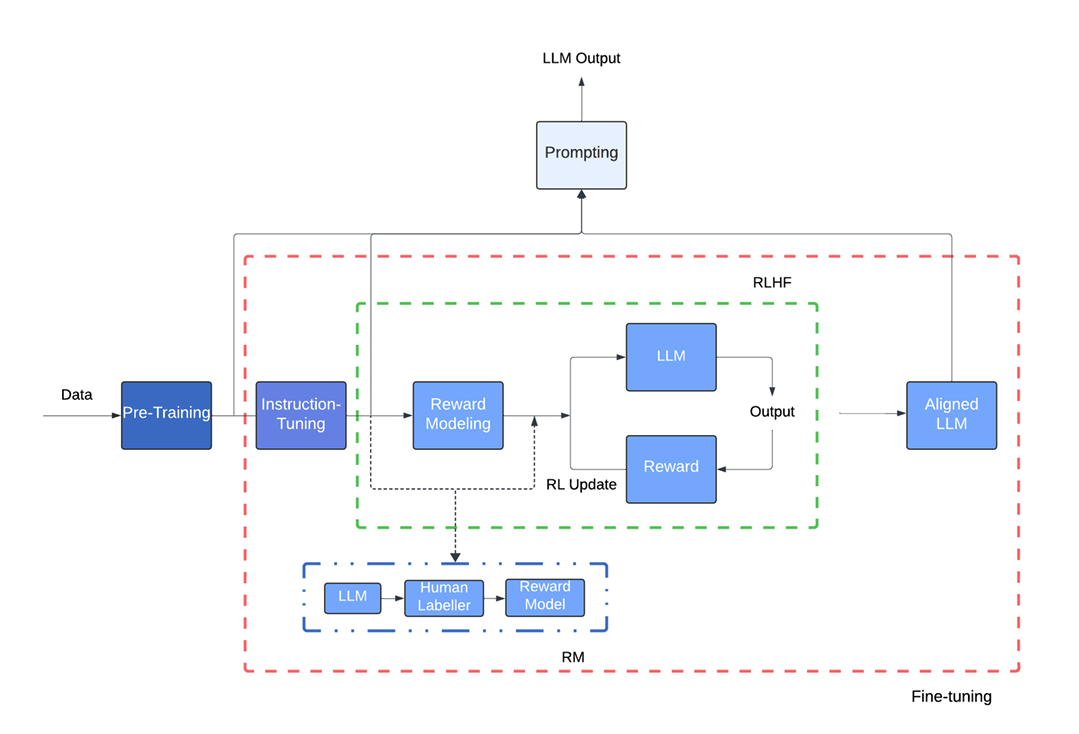
\includegraphics[width=\linewidth]{immagini/pre-training-e-fine-tuning.png}
    \caption{Diagramma del flusso delle fasi di addestramento di un LLM, dalla fase di pre-training fino alla generazione tramite prompt.\cite{hadi_2024}}
    \label{fig:example}
\end{figure}

\subsection{Scalabilità e parametri del modello}
La scalabilità è uno degli aspetti chiave che ha permesso agli LLM di raggiungere livelli di prestazione straordinari. Con il termine "scalabilità" ci si riferisce alla capacità di un modello di gestire un numero sempre maggiore di parametri, che sono i valori numerici che il modello apprende durante l’addestramento. Un aumento nel numero di parametri consente al modello di rappresentare e processare con maggiore precisione informazioni linguistiche complesse, migliorando la sua capacità di comprendere e generare testo.\cite{hadi_2024}

\subsubsection{Il ruolo dei parametri nell'evoluzione degli LLM}
I primi modelli di linguaggio, come GPT-2, operavano con centinaia di milioni di parametri. Tuttavia, con l’evoluzione dei modelli, si è passati a miliardi e persino centinaia di miliardi di parametri. Ad esempio, GPT-3, uno dei modelli più avanzati al momento del suo rilascio, conta 175 miliardi di parametri, mentre modelli successivi, come GPT-4, utilizzano dataset ancora più vasti e un numero di parametri più che doppio. Questo aumento esponenziale consente al modello di catturare sfumature semantiche e relazioni tra parole su scala globale, migliorando la sua capacità di risolvere task complessi e diversificati.\cite{zhao_2023}

\subsubsection{Il Ruolo dei Dati: disponibilità e limiti}
Un aspetto cruciale nell'addestramento degli LLM riguarda la quantità e la qualità dei dati disponibili. Si prevede che, entro la fine di questo decennio, l’intera disponibilità di dati testuali generati dall’uomo potrebbe essere utilizzata per l'addestramento dei modelli, creando una situazione di "bottleneck" legata ai dati. Secondo stime recenti, se le tendenze attuali di sviluppo continuano, i dataset utilizzati per l’addestramento potrebbero esaurire l'intero stock di dati pubblici testuali tra il 2026 e il 2032.
Con l'aumento delle dimensioni dei modelli e della quantità di dati necessari, l’industria si trova di fronte alla sfida di reperire nuove fonti di dati. Una volta esauriti i dati pubblici disponibili, che costituiscono la base principale per l'addestramento attuale, resta ancora un'enorme quantità di conoscenza derivabile da fonti non pubbliche o dal deep web, ossia il web non indicizzato e non accessibile tramite i motori di ricerca tradizionali. Secondo alcune stime, il deep web e i dati non pubblici, come le conversazioni nelle app di messaggistica istantanea e nei social media privati, potrebbero contenere fino a un quadrilione di token, una quantità comparabile all'intero web indicizzato. Inoltre, si sta esplorando l'uso di dati provenienti da fonti non testuali come immagini, video e audio, che possono essere integrati per arricchire l'addestramento dei modelli. Tuttavia, l’accesso e l’utilizzo di questi dati pongono sfide significative, tra cui questioni legali, di privacy e la qualità spesso inferiore rispetto ai dati pubblici, con potenziali rischi per la robustezza dei modelli.\cite{villalobos_2024}

\subsubsection{Innovazioni per la scalabilità e la qualità dei dati}
Per superare i limiti legati alla scarsità di dati testuali generati dall’uomo, la ricerca sta esplorando diverse soluzioni innovative. Tra queste, l’uso di dati sintetici generati dagli stessi modelli LLM si sta rivelando promettente. Questi dati sintetici possono essere creati per coprire gap specifici nei dataset esistenti, migliorando la diversità e la qualità delle informazioni disponibili.\cite{villalobos_2024} Un’altra linea di sviluppo è l’apprendimento multimodale, che permette ai modelli di integrare dati provenienti da fonti diverse, come immagini, video e audio. Questa fusione di modalità non solo arricchisce le capacità del modello, ma offre anche nuove prospettive di addestramento, sfruttando informazioni non linguistiche per potenziare la comprensione contestuale e semantica.\cite{naveed_2024}

\subsection{Sfide computazionali e soluzioni per la scalabilità degli LLM}
Sebbene l’aumento dei parametri abbia portato a miglioramenti significativi nelle prestazioni degli LLM, ha anche introdotto sfide tecniche e logistiche notevoli. Addestrare un modello con centinaia di miliardi di parametri richiede risorse computazionali immense: l’addestramento di modelli come GPT-3, ad esempio, ha richiesto petaflop/s di potenza di calcolo per settimane, con costi stimati in milioni di dollari. Questi processi coinvolgono l’utilizzo di GPU e TPU di ultima generazione distribuite su cluster di larga scala. Inoltre, l’alto consumo energetico e la gestione di infrastrutture complesse pongono sfide logistiche significative.\cite{hadi_2024}

Nonostante l’espansione dei parametri migliori le capacità del modello, l’incremento non sempre si traduce in benefici lineari: superati certi livelli, i miglioramenti diventano marginali, rendendo necessario un bilanciamento attento tra la dimensione del modello e i vantaggi reali ottenuti. Per affrontare queste sfide, sono state sviluppate tecniche ad hoc, come la sparse attention che consente al modello di focalizzarsi solo su una parte selezionata delle informazioni, riducendo così il numero di operazioni e ottimizzando il costo computazionale, o i modelli Mixture-of-Experts (MoE) che attivano solo una porzione del modello per processare ogni input, distribuendo la complessità su diverse sottoreti e permettendo di scalare ulteriormente i parametri senza doverli utilizzare tutti contemporaneamente.\cite{naveed_2024}

\section{Generazione di testo e prompt engineering}
Uno degli aspetti centrali nell’uso pratico dei Large Language Models (LLM) è il modo in cui si formulano e ottimizzano i prompt per ottenere risposte di alta qualità. Questo processo, noto come prompt engineering, si basa sulla capacità di sfruttare al meglio le potenzialità del modello attraverso istruzioni precise e ben strutturate fornite in linguaggio naturale. Il prompt engineering rappresenta l’arte e la scienza di formulare input specifici per i modelli linguistici di grandi dimensioni (LLM) al fine di ottenere risposte precise, contestualizzate e rilevanti. Questo processo è cruciale perché, nonostante la sofisticatezza degli LLM, l'efficacia delle risposte dipende fortemente dalla chiarezza, specificità e struttura del prompt. Un buon prompt può fare la differenza tra una risposta generica e una risposta dettagliata e pertinente, permettendo al modello di sfruttare appieno le sue capacità. Le linee guida, le tecniche e i parametri specifici del modello sono tutti elementi essenziali per massimizzare i risultati. L’arte di formulare un buon prompt può determinare il successo nell’ottenere risultati di qualità e nell’adattare la generazione di testo alle necessità specifiche dell’utente.\cite{sahoo_2024}\cite{zhao_2023}

\subsection{Linee guida per un buon prompt}
Per ottenere risultati precisi e pertinenti dai modelli di linguaggio, è essenziale progettare prompt chiari e ben strutturati. Un buon prompt deve fornire le giuste informazioni, contestualizzare il task e definire chiaramente le aspettative. Di seguito sono descritte le linee guida principali per massimizzare l'efficacia dei prompt.\cite{vogelsang_2024}\cite{chen_2023}

\subsubsection{Fornire contesto}
È fondamentale includere informazioni contestuali che possano orientare il modello nella generazione di risposte appropriate. Il contesto può riguardare il tema trattato, il tipo di pubblico a cui è destinato il contenuto o eventuali prerequisiti da considerare. Un contesto ben definito consente al modello di allineare meglio le sue risposte con le aspettative dell’utente.

\subsubsection{Istruzioni dettagliate}
Un prompt deve essere accompagnato da istruzioni precise che descrivano in maniera dettagliata il compito richiesto. In questo modo, il modello riceve indicazioni chiare sul tipo di output da generare, minimizzando l'ambiguità e migliorando la pertinenza della risposta. È consigliabile utilizzare verbi che esprimano azioni concrete e dirette, come "analizzare", "descrivere", o "sintetizzare".

\subsubsection{Definizione di un ruolo per il modello}
Attribuire un ruolo specifico al modello è una strategia utile per ottenere risposte più focalizzate e coerenti. Definire il modello come un esperto in un determinato settore o come un interlocutore che si rivolge a un pubblico specifico permette di adattare il tono e la struttura dell’output generato, migliorando la qualità complessiva della risposta.

\subsubsection{Specifiche dell’output}
Stabilire in modo esplicito le caratteristiche dell’output desiderato, come il formato, la lunghezza o la struttura, è essenziale per guidare il modello verso una produzione testuale conforme alle necessità dell’utente. Indicare con precisione il numero di parole, frasi o paragrafi, così come l’eventuale suddivisione in elenchi puntati o sezioni, contribuisce a rendere l’output più adeguato al contesto di utilizzo.

\subsubsection{Definizione di regole e vincoli}
Un buon prompt può includere regole specifiche o vincoli da rispettare durante la generazione del testo. Tali regole possono riguardare, ad esempio, il mantenimento di un certo registro linguistico, l’esclusione di determinate informazioni o l’adozione di un particolare stile narrativo. L’imposizione di questi vincoli consente di affinare ulteriormente l’output e di adattarlo a specifiche esigenze di comunicazione.

\subsection{Tecniche avanzate di prompt engineering}
Oltre alle linee guida di base per la progettazione di prompt efficaci, esistono strategie avanzate che permettono di gestire task complessi, sfruttare capacità multimodali e migliorare il ragionamento del modello. Queste tecniche sono particolarmente utili in contesti che richiedono un elevato grado di precisione o l'integrazione di informazioni provenienti da fonti diverse.

\subsubsection{Divisione dei task complessi}
In presenza di task articolati o con più fasi, suddividere il problema in sotto-task più gestibili consente di guidare il modello in modo progressivo. Questo approccio prevede l'uso di prompt sequenziali che richiedono al modello di affrontare un passo alla volta, facilitando la gestione di attività complesse e migliorando la qualità complessiva dell’output. La scomposizione permette anche di verificare l’accuratezza delle risposte in ogni fase, prima di procedere al passaggio successivo.

\subsubsection{Utilizzo di modelli multimodali}
I modelli multimodali sono progettati per elaborare input provenienti da più domini, come testo, immagini, audio e video, e generare output integrati. Questa capacità estende l'utilità dei modelli di linguaggio a scenari in cui è necessaria la combinazione di dati eterogenei. Nella progettazione di prompt per questi modelli, è cruciale specificare chiaramente il tipo di input desiderato e le modalità con cui le informazioni devono essere correlate, per ottenere risposte coerenti e complete.

\subsubsection{Socratic prompting}
Il Socratic Prompting è una tecnica che si ispira al metodo socratico, basato sull'uso di domande successive per stimolare il ragionamento e l’approfondimento. Questa strategia prevede una serie di domande mirate, progettate per guidare il modello nell’esplorazione di un concetto complesso attraverso risposte progressive. Il vantaggio di questo approccio risiede nella capacità di esplorare il problema da più angolazioni, favorendo l’emergere di risposte più articolate e riflessive.

\subsection{Tecniche di prompt per l'ottimizzazione dei modelli di linguaggio}
Nell’ambito dell’ingegneria dei prompt, esistono diverse tecniche che permettono di guidare i modelli di linguaggio a seconda del tipo di task e del livello di complessità richiesto. Le principali tecniche sono illustrate di seguito.\cite{sahoo_2024}

\subsubsection{Zero-Shot prompting}
Zero-shot prompting è una tecnica in cui il modello di linguaggio viene sollecitato a rispondere senza fornire esempi specifici relativi al compito richiesto. In questa configurazione, il modello si affida unicamente alla sua capacità generale di comprensione per generare un output appropriato. Questa tecnica è utile in scenari in cui non sono disponibili esempi predefiniti o quando si cerca una risposta basata unicamente sulla conoscenza pre-allenata del modello.

\subsubsection{One-Shot prompting}
Con il one-shot prompting, si include un singolo esempio all’interno del prompt per indicare al modello la struttura o la logica della risposta desiderata. L’aggiunta di un esempio permette al modello di adattare meglio il suo output, migliorando la precisione rispetto al contesto specifico. Questo metodo è particolarmente utile per task che richiedono un format o uno stile specifico, dove anche un solo esempio può fare la differenza.

\subsubsection{Few-Shot prompting}
Il few-shot prompting si basa sull’inclusione di più esempi all’interno del prompt. Questa tecnica consente al modello di osservare e generalizzare pattern più complessi, migliorando la coerenza e l’affidabilità dell’output per task articolati. Il few-shot prompting è ampiamente utilizzato per task come il completamento di frasi, la traduzione automatica e il riassunto, dove un contesto esteso aiuta il modello a cogliere meglio le sfumature del compito.

\subsubsection{Multi-Shot prompting}
Il multi-shot prompting estende ulteriormente il numero di esempi forniti al modello, permettendo di affrontare task molto complessi. Fornendo un’ampia gamma di esempi, il modello riesce a raffinare la propria comprensione e a produrre risposte dettagliate e articolate. Questa tecnica è adatta a contesti in cui la varietà di casi di input richiede un approccio flessibile e altamente adattabile.

\subsubsection{Chain-of-Thought Prompting (CoT)}
Il chain-of-thought prompting è una tecnica avanzata in cui il modello viene guidato a suddividere un problema complesso in passaggi logici sequenziali. Questa strategia sfrutta la capacità del modello di sviluppare un ragionamento articolato attraverso una serie di step interconnessi. Il CoT è particolarmente utile per task che richiedono deduzione, ragionamento matematico o problemi multi-step, dove la sequenza logica degli argomenti è fondamentale per arrivare a una soluzione corretta.

\subsubsection{Zero-Shot Chain-of-Thought (CoT) Prompting}
Il zero-shot chain-of-thought prompting combina l’approccio zero-shot con la logica del chain-of-thought. In questa configurazione, il modello è incoraggiato a generare un ragionamento sequenziale senza la necessità di fornire esempi espliciti. Il modello è indotto a creare autonomamente un flusso di pensieri articolato, guidando la risoluzione del task attraverso una serie di passaggi logici, anche quando non è stato addestrato su task specifici che coinvolgono tali processi.

\subsection{Configurazione dei parametri per l’ottimizzazione della generazione del testo}
Nell’interazione con modelli di linguaggio di grandi dimensioni (LLM), la configurazione dei parametri tecnici è fondamentale per controllare e ottimizzare la qualità dell’output generato. Ogni parametro regola aspetti diversi del comportamento del modello, influenzando sia la creatività che la coerenza delle risposte. È importante comprendere il range di valori disponibili per ciascun parametro e come questi possono essere modulati per ottenere risultati desiderabili. Di seguito vengono descritti i principali parametri configurabili, illustrando prima i range operativi e poi l’effetto che valori specifici possono avere sulla generazione del testo.\cite{zhao_2023}\cite{naveed_2024}

\subsubsection{Temperatura}
Il parametro della temperatura controlla il grado di casualità nell’output generato. Il range tipico varia tra 0 e 1. Con valori vicini allo 0, il modello tende a essere deterministico, generando risposte prevedibili e concrete, selezionando sempre il token più probabile. Al contrario, valori prossimi a 1 aumentano l’esplorazione di token meno frequenti, favorendo la creatività.
Valori bassi della temperatura, tra 0.0 e 0.3, sono ideali per compiti in cui è richiesta precisione, come il question answering basato sui fatti o la sintesi di informazioni, dove è preferibile che l’output sia concreto e privo di variabilità. Valori intermedi, tra 0.4 e 0.7, rappresentano un compromesso tra creatività e precisione, adattandosi a contesti dove è richiesta una certa flessibilità nella risposta. Infine, valori alti, tra 0.8 e 1.0, sono indicati per la generazione di testi creativi, come racconti, poesie o contenuti in cui l’originalità e la varietà sono più importanti della coerenza assoluta.

\subsubsection{Top P (Campionamento del Nucleo)}
Il parametro \textit{top\_p}, noto anche come campionamento del nucleo, definisce il sottoinsieme di token da cui il modello può scegliere durante la generazione del testo. Il range varia tra 0 e 1. Con valori bassi, ad esempio 0.2 o 0.3, vengono considerati solo i token con le probabilità più alte, producendo risposte sicure e prevedibili. Valori più alti, come 0.8 o 0.9, permettono al modello di esplorare opzioni meno comuni, generando un output più variegato.
Quando \textit{top\_p} è impostato a 1, il modello considera tutti i token possibili, producendo risposte altamente creative ma potenzialmente incoerenti. Se si desidera un output preciso e mirato, si consiglia di mantenere \textit{top\_p} tra 0.2 e 0.4. In contesti in cui è importante ottenere risposte diverse e creative, è preferibile impostare \textit{top\_p} tra 0.7 e 0.9. È importante notare che, in molti casi, è consigliabile modificare la temperatura o \textit{top\_p}, ma non entrambi contemporaneamente, per mantenere un controllo efficace sull’output generato.

\subsubsection{Lunghezza Massima}
La lunghezza massima specifica il numero massimo di token che il modello può generare. Un token è l’unità di misura usata dal LLM per definire la lunghezza del testo. Un token può essere un carattere singolo, una parola completa o parte di una parola, a seconda del contesto e della lingua utilizzata. Questo parametro è essenziale per evitare risposte eccessivamente prolisse o fuori tema, e per ottimizzare i costi computazionali. Ogni modello ha un limite massimo di token, che varia a seconda della specifica implementazione. La configurazione della lunghezza massima dipende strettamente dalla natura del task e dal livello di dettaglio richiesto.

\subsubsection{Sequenze di Stop}
Le sequenze di stop sono stringhe specifiche che indicano al modello quando interrompere la generazione del testo, contribuendo così a migliorare la struttura e la coerenza dell’output. Questo parametro risulta particolarmente utile in contesti in cui è necessario controllare la lunghezza della risposta o segmentare l’output in sezioni ben definite. Ad esempio, in un elenco puntato, le sequenze di stop possono essere impiegate per evitare che il modello generi più voci del necessario, mantenendo il testo all’interno dei limiti desiderati. L’utilizzo di questo parametro è consigliato quando si richiede una risposta breve e mirata, come in applicazioni di chatbot o risposte a domande specifiche, dove l'output deve fermarsi dopo aver fornito l'informazione essenziale. In contesti in cui è preferibile ottenere una risposta più completa e articolata, potrebbe non essere necessario configurare le sequenze di stop, permettendo al modello di generare un output che esaurisca l’argomento richiesto.

\subsubsection{Penalità di Frequenza}
La penalità di frequenza regola la probabilità che il modello ripeta lo stesso token più volte all’interno dell’output generato. Questo parametro varia tipicamente da 0 a 2. Con valori più alti, come 0.8 o 1.0, la probabilità di ripetizione diminuisce, favorendo una maggiore diversificazione del testo generato. Valori più bassi, tra 0.2 e 0.5, consentono un certo grado di ripetizione, utile in contesti in cui la coerenza del discorso è prioritaria.

\subsubsection{Penalità di Presenza}
Simile alla penalità di frequenza, la penalità di presenza influenza la probabilità che il modello ripeta i token, ma lo fa in modo uniforme, indipendentemente dal numero di occorrenze precedenti di un dato token. Con valori alti, tipicamente tra 0.6 e 0.8, la penalità di presenza riduce la ripetizione dei token, migliorando la varietà dell’output e rendendolo più dinamico. Questo è utile in scenari in cui si desidera mantenere l’originalità e l’interesse del testo, come nella generazione di contenuti creativi o nell’elaborazione di risposte complesse che richiedono una certa diversificazione linguistica.
Al contrario, valori bassi di penalità di presenza, tra 0.1 e 0.3, sono indicati quando si necessita di una maggiore continuità tematica e coesione nel testo, come in articoli accademici o in documenti tecnici, dove la ripetizione di termini specifici può essere essenziale per mantenere la chiarezza e la precisione dell’argomentazione. 


\subsection{Problematiche della generazione del testo}
Nonostante i progressi significativi ottenuti con i modelli di linguaggio di grandi dimensioni (LLM), la generazione automatica del testo presenta ancora diverse problematiche critiche che ne limitano l’applicabilità in contesti che richiedono affidabilità e precisione. Di seguito vengono analizzati i principali ostacoli che emergono durante l’uso di LLM in diversi scenari applicativi.

\subsubsection{Allucinazioni nei Modelli di Linguaggio}
Uno dei principali limiti degli LLM è la tendenza a generare informazioni false o non pertinenti, fenomeno noto come “allucinazione”. Queste allucinazioni si verificano quando il modello produce contenuti apparentemente plausibili ma che non corrispondono a fatti reali o informazioni verificate. Le allucinazioni possono essere distinte in due categorie principali: intrinseche ed estrinseche. Le allucinazioni intrinseche si verificano quando il modello produce contenuti che, pur essendo plausibili e ben formati dal punto di vista linguistico, non sono basati su dati reali o verificabili. Questi errori derivano dalla natura stessa del modello, che può combinare o inferire informazioni errate durante la generazione del testo. Le allucinazioni estrinseche, invece, si manifestano quando il modello tenta di rispondere a domande o seguire prompt per i quali non ha sufficienti informazioni nel dataset di addestramento o quando il contesto fornito è ambiguo o insufficiente. Questo tipo di allucinazione è particolarmente pericoloso in settori che richiedono un elevato grado di accuratezza, come la ricerca scientifica, la medicina o il diritto.
Affrontare queste problematiche richiede un’attenta progettazione dei prompt, nonché l’integrazione di meccanismi di verifica che possano limitare le allucinazioni, specialmente quelle estrinseche, attraverso il recupero di informazioni aggiornate da fonti esterne. In questo contesto, l’approccio Retrieval-Augmented Generation (RAG) rappresenta una soluzione promettente. Il RAG combina la generazione del testo con il recupero di informazioni esterne durante l’elaborazione, permettendo al modello di consultare fonti aggiornate e pertinenti. Ciò riduce il rischio di allucinazioni e migliora l’accuratezza delle risposte, soprattutto in domini dove l’aggiornamento continuo delle informazioni è fondamentale.\cite{ji_2023}

\subsubsection{Coerenza e coesione del discorso}
Un’altra sfida riguarda la capacità del modello di mantenere la coerenza tematica e stilistica all'interno di testi più lunghi o complessi. In task complessi o in testi più lunghi, i modelli possono perdere il filo logico del discorso, producendo output che risultano disorganizzati o incoerenti rispetto al contesto iniziale. Questo è spesso dovuto all’incapacità del modello di gestire correttamente il contesto a lungo termine. Questa limitazione diventa evidente in testi argomentativi o narrativi, dove il modello può deviare dal tema centrale, generando informazioni non pertinenti o ripetitive. La gestione efficace del contesto a lungo termine rimane una sfida aperta per la ricerca, richiedendo soluzioni che combinino la modellazione del discorso con strategie di memoria più avanzate.\cite{naveed_2024}

\subsubsection{Bias nei dati e riproduzione di stereotipi}
Gli LLM, essendo addestrati su grandi quantità di dati non supervisionati, possono riprodurre bias e stereotipi presenti nel corpus di addestramento. Questi bias possono emergere nella generazione del testo sotto forma di pregiudizi impliciti o generalizzazioni inadeguate, con implicazioni etiche rilevanti quando il modello viene utilizzato in contesti sensibili. Sebbene esistano tecniche di mitigazione dei bias, come il fine-tuning su dati diversificati o l’applicazione di filtri etici, la piena eliminazione di questi effetti rimane complessa e richiede un monitoraggio continuo del comportamento del modello.\cite{hadi_2024}

\subsubsection{Aderenza alle istruzioni e comprensione del prompt}
L’efficacia del prompting dipende in gran parte dalla capacità del modello di interpretare correttamente le istruzioni fornite. Sebbene tecniche come il few-shot o il chain-of-thought prompting possano migliorare la comprensione del compito, i modelli spesso faticano a seguire istruzioni articolate o a rispondere a prompt complessi che richiedono risoluzioni multi-step. Questo problema si aggrava in presenza di ambiguità o di richieste multiple all'interno dello stesso prompt, portando il modello a generare output incompleti o non conformi alle aspettative. Per ovviare a questa limitazione, è necessario affinare la progettazione dei prompt e, in alcuni casi, ricorrere a un’interazione iterativa con il modello per ottenere il risultato desiderato.\cite{sahoo_2024}

\subsubsection{Limitazioni nel ragionamento e nella pianificazione}
Nonostante le loro capacità avanzate nella generazione del linguaggio naturale, i modelli di linguaggio di grandi dimensioni (LLM) mostrano evidenti limitazioni quando si tratta di compiti che richiedono ragionamento e pianificazione complessi. Sebbene possano sembrare in grado di affrontare compiti di ragionamento superficiale, gli LLM mancano delle capacità necessarie per gestire situazioni che richiedono una comprensione profonda e una pianificazione basata sul buon senso, attività che per gli esseri umani risultano spesso intuitive. Questo limite deriva dal fatto che gli LLM generano completamenti di testo basati su probabilità statistiche piuttosto che su processi logici strutturati. Di conseguenza, in contesti che richiedono deduzione, pianificazione strategica o la risoluzione di problemi multi-step, gli LLM tendono a fallire, producendo risposte che possono essere incoerenti o prive di logica.\cite{naveed_2024}

% Capitolo
\chapter{Design della soluzione}
In hac habitasse platea dictumst. Vestibulum consectetur dictum pellentesque. Suspendisse nunc neque, commodo ac imperdiet nec, sollicitudin vitae libero. Donec bibendum vel nunc vitae pharetra. In vel volutpat odio, et interdum dui. Duis mauris ligula, congue eget molestie at, tincidunt nec diam. Nam vitae eros nec arcu suscipit vehicula. Aliquam consectetur imperdiet elit, eget pretium arcu fringilla at. Maecenas sed libero pulvinar, mattis tortor vel, fermentum enim.

%% Sezione
\section{Titolo della Sezione}
Donec pulvinar neque non lectus vulputate pellentesque. Quisque rutrum arcu velit, in feugiat sapien posuere vel. Praesent metus orci, aliquam ac cursus eget, fermentum a nisl. Etiam eu augue lacus. Nam nisi sapien, mattis sed vehicula non, pellentesque at quam. Sed euismod, dolor nec commodo lobortis, erat erat ultricies eros, bibendum dictum nulla felis in dui. Nulla blandit ultrices arcu, vitae lacinia tellus tempor sit amet. Nulla non tincidunt dolor. In eget luctus sem, sed elementum ligula. Proin elementum adipiscing sem, sit amet ultricies nisl tincidunt eu. Ut lobortis dui quam, et scelerisque erat ultrices sit amet. Sed libero sem, mollis quis euismod quis, suscipit ac justo.

%% Sottosezione
\subsection{Sottosezione}
Donec cursus tortor eget sem ornare imperdiet. Ut vel orci non ipsum condimentum laoreet vitae ut sapien. Aenean metus mi, vehicula quis turpis nec, porttitor blandit dui. Nullam sed sollicitudin quam. Fusce nisl ante, commodo eget lacus ac, mollis ullamcorper neque. Quisque faucibus dictum nisl, dignissim fermentum sapien fringilla vel. Proin dui velit, molestie sit amet sapien et, pellentesque tristique purus. Curabitur ac quam ac diam varius bibendum.

%% Capitolo
\chapter{Design dell'esperimento}
In hac habitasse platea dictumst. Vestibulum consectetur dictum pellentesque. Suspendisse nunc neque, commodo ac imperdiet nec, sollicitudin vitae libero. Donec bibendum vel nunc vitae pharetra. In vel volutpat odio, et interdum dui. Duis mauris ligula, congue eget molestie at, tincidunt nec diam. Nam vitae eros nec arcu suscipit vehicula. Aliquam consectetur imperdiet elit, eget pretium arcu fringilla at. Maecenas sed libero pulvinar, mattis tortor vel, fermentum enim.

%% Sezione
\section{Titolo della Sezione}
Donec pulvinar neque non lectus vulputate pellentesque. Quisque rutrum arcu velit, in feugiat sapien posuere vel. Praesent metus orci, aliquam ac cursus eget, fermentum a nisl. Etiam eu augue lacus. Nam nisi sapien, mattis sed vehicula non, pellentesque at quam. Sed euismod, dolor nec commodo lobortis, erat erat ultricies eros, bibendum dictum nulla felis in dui. Nulla blandit ultrices arcu, vitae lacinia tellus tempor sit amet. Nulla non tincidunt dolor. In eget luctus sem, sed elementum ligula. Proin elementum adipiscing sem, sit amet ultricies nisl tincidunt eu. Ut lobortis dui quam, et scelerisque erat ultrices sit amet. Sed libero sem, mollis quis euismod quis, suscipit ac justo.

%% Sottosezione
\subsection{Sottosezione}
Donec cursus tortor eget sem ornare imperdiet. Ut vel orci non ipsum condimentum laoreet vitae ut sapien. Aenean metus mi, vehicula quis turpis nec, porttitor blandit dui. Nullam sed sollicitudin quam. Fusce nisl ante, commodo eget lacus ac, mollis ullamcorper neque. Quisque faucibus dictum nisl, dignissim fermentum sapien fringilla vel. Proin dui velit, molestie sit amet sapien et, pellentesque tristique purus. Curabitur ac quam ac diam varius bibendum.

%% Capitolo
\chapter{Conclusioni e sviluppi futuri}
In hac habitasse platea dictumst. Vestibulum consectetur dictum pellentesque. Suspendisse nunc neque, commodo ac imperdiet nec, sollicitudin vitae libero. Donec bibendum vel nunc vitae pharetra. In vel volutpat odio, et interdum dui. Duis mauris ligula, congue eget molestie at, tincidunt nec diam. Nam vitae eros nec arcu suscipit vehicula. Aliquam consectetur imperdiet elit, eget pretium arcu fringilla at. Maecenas sed libero pulvinar, mattis tortor vel, fermentum enim.

%% Sezione
\section{Titolo della Sezione}
Donec pulvinar neque non lectus vulputate pellentesque. Quisque rutrum arcu velit, in feugiat sapien posuere vel. Praesent metus orci, aliquam ac cursus eget, fermentum a nisl. Etiam eu augue lacus. Nam nisi sapien, mattis sed vehicula non, pellentesque at quam. Sed euismod, dolor nec commodo lobortis, erat erat ultricies eros, bibendum dictum nulla felis in dui. Nulla blandit ultrices arcu, vitae lacinia tellus tempor sit amet. Nulla non tincidunt dolor. In eget luctus sem, sed elementum ligula. Proin elementum adipiscing sem, sit amet ultricies nisl tincidunt eu. Ut lobortis dui quam, et scelerisque erat ultrices sit amet. Sed libero sem, mollis quis euismod quis, suscipit ac justo.

%% Sottosezione
\subsection{Sottosezione}
Donec cursus tortor eget sem ornare imperdiet. Ut vel orci non ipsum condimentum laoreet vitae ut sapien. Aenean metus mi, vehicula quis turpis nec, porttitor blandit dui. Nullam sed sollicitudin quam. Fusce nisl ante, commodo eget lacus ac, mollis ullamcorper neque. Quisque faucibus dictum nisl, dignissim fermentum sapien fringilla vel. Proin dui velit, molestie sit amet sapien et, pellentesque tristique purus. Curabitur ac quam ac diam varius bibendum.


%% Fine dei capitoli normali, inizio dei capitoli-appendice (opzionali)
\appendix

%\part{Appendici}

\chapter{Titolo della prima appendice}
Sed purus libero, vestibulum ut nibh vitae, mollis ultricies augue. Pellentesque velit libero, tempor sed pulvinar non, fermentum eu leo. Duis posuere eleifend nulla eget sagittis. Nam laoreet accumsan rutrum. Interdum et malesuada fames ac ante ipsum primis in faucibus. Curabitur eget libero quis leo porttitor vehicula eget nec odio. Proin euismod interdum ligula non ultricies. Maecenas sit amet accumsan sapien.

%% Parte conclusiva del documento; tipicamente per riassunto, bibliografia e/o indice analitico.
\backmatter

%% Riassunto (opzionale)
%\summary
%Maecenas tempor elit sed arcu commodo, dapibus sagittis leo egestas. Praesent at ultrices urna. Integer et nibh in augue mollis facilisis sit amet eget magna. Fusce at porttitor sapien. Phasellus imperdiet, felis et molestie vulputate, mauris sapien tincidunt justo, in lacinia velit nisi nec ipsum. Duis elementum pharetra lorem, ut pellentesque nulla congue et. Sed eu venenatis tellus, pharetra cursus felis. Sed et luctus nunc. Aenean commodo, neque a aliquam bibendum, mauris augue fringilla justo, et scelerisque odio mi sit amet diam. Nulla at placerat nibh, nec rutrum urna. Donec ut egestas magna. Aliquam erat volutpat. Phasellus vestibulum justo sed purus mattis, vitae lacinia magna viverra. Nulla rutrum diam dui, vel semper mi mattis ac. Vestibulum ante ipsum primis in faucibus orci luctus et ultrices posuere cubilia Curae; Donec id vestibulum lectus, eget tristique est.

%% Bibliografia (praticamente obbligatoria)
\bibliographystyle{plain_\languagename}%% Carica l'omonimo file .bst, dove \languagename è la lingua attiva.
%% Nel caso in cui si usi un file .bib (consigliato)
\bibliography{thesis_bibliography}
%% Nel caso di bibliografia manuale, usare l'environment thebibliography.

%% Per l'indice analitico, usare il pacchetto makeidx (o analogo).

\end{document}

--- Istruzioni per l'aggiunta di nuove lingue ---
Per ogni nuova lingua utilizzata aggiungere nel preambolo il seguente spezzone:
    \addto\captionsitalian{%
        \def\abstractname{Sommario}%
        \def\acknowledgementsname{Ringraziamenti}%
        \def\authorcontactsname{Contatti dell'autore}%
        \def\candidatename{Candidato}%
        \def\chairname{Direttore}%
        \def\conclusionsname{Conclusioni}%
        \def\cosupervisorname{Co-relatore}%
        \def\cosupervisorsname{Co-relatori}%
        \def\cyclename{Ciclo}%
        \def\datename{Anno accademico}%
        \def\indexname{Indice analitico}%
        \def\institutecontactsname{Contatti dell'Istituto}%
        \def\introductionname{Introduzione}%
        \def\prefacename{Prefazione}%
        \def\reviewername{Controrelatore}%
        \def\reviewersname{Controrelatori}%
        %% Anno accademico
        \def\shortdatename{A.A.}%
        \def\summaryname{Riassunto}%
        \def\supervisorname{Relatore}%
        \def\supervisorsname{Relatori}%
        \def\thesisname{Tesi di \expandafter\ifcase\csname thud@target\endcsname Laurea\or Laurea Magistrale\or Dottorato\fi}%
        \def\tutorname{Tutor aziendale%
        \def\tutorsname{Tutor aziendali}%
    }
sostituendo a "italian" (nella 1a riga) il nome della lingua e traducendo le varie voci.
